% Options for packages loaded elsewhere
\PassOptionsToPackage{unicode}{hyperref}
\PassOptionsToPackage{hyphens}{url}
%
\documentclass[
]{article}
\usepackage{lmodern}
\usepackage{amssymb,amsmath}
\usepackage{ifxetex,ifluatex}
\ifnum 0\ifxetex 1\fi\ifluatex 1\fi=0 % if pdftex
  \usepackage[T1]{fontenc}
  \usepackage[utf8]{inputenc}
  \usepackage{textcomp} % provide euro and other symbols
\else % if luatex or xetex
  \usepackage{unicode-math}
  \defaultfontfeatures{Scale=MatchLowercase}
  \defaultfontfeatures[\rmfamily]{Ligatures=TeX,Scale=1}
\fi
% Use upquote if available, for straight quotes in verbatim environments
\IfFileExists{upquote.sty}{\usepackage{upquote}}{}
\IfFileExists{microtype.sty}{% use microtype if available
  \usepackage[]{microtype}
  \UseMicrotypeSet[protrusion]{basicmath} % disable protrusion for tt fonts
}{}
\makeatletter
\@ifundefined{KOMAClassName}{% if non-KOMA class
  \IfFileExists{parskip.sty}{%
    \usepackage{parskip}
  }{% else
    \setlength{\parindent}{0pt}
    \setlength{\parskip}{6pt plus 2pt minus 1pt}}
}{% if KOMA class
  \KOMAoptions{parskip=half}}
\makeatother
\usepackage{xcolor}
\IfFileExists{xurl.sty}{\usepackage{xurl}}{} % add URL line breaks if available
\IfFileExists{bookmark.sty}{\usepackage{bookmark}}{\usepackage{hyperref}}
\hypersetup{
  pdftitle={Empirical calibration of confidence intervals},
  pdfauthor={Martijn J. Schuemie, Marc A. Suchard},
  hidelinks,
  pdfcreator={LaTeX via pandoc}}
\urlstyle{same} % disable monospaced font for URLs
\usepackage[margin=1in]{geometry}
\usepackage{color}
\usepackage{fancyvrb}
\newcommand{\VerbBar}{|}
\newcommand{\VERB}{\Verb[commandchars=\\\{\}]}
\DefineVerbatimEnvironment{Highlighting}{Verbatim}{commandchars=\\\{\}}
% Add ',fontsize=\small' for more characters per line
\usepackage{framed}
\definecolor{shadecolor}{RGB}{248,248,248}
\newenvironment{Shaded}{\begin{snugshade}}{\end{snugshade}}
\newcommand{\AlertTok}[1]{\textcolor[rgb]{0.94,0.16,0.16}{#1}}
\newcommand{\AnnotationTok}[1]{\textcolor[rgb]{0.56,0.35,0.01}{\textbf{\textit{#1}}}}
\newcommand{\AttributeTok}[1]{\textcolor[rgb]{0.77,0.63,0.00}{#1}}
\newcommand{\BaseNTok}[1]{\textcolor[rgb]{0.00,0.00,0.81}{#1}}
\newcommand{\BuiltInTok}[1]{#1}
\newcommand{\CharTok}[1]{\textcolor[rgb]{0.31,0.60,0.02}{#1}}
\newcommand{\CommentTok}[1]{\textcolor[rgb]{0.56,0.35,0.01}{\textit{#1}}}
\newcommand{\CommentVarTok}[1]{\textcolor[rgb]{0.56,0.35,0.01}{\textbf{\textit{#1}}}}
\newcommand{\ConstantTok}[1]{\textcolor[rgb]{0.00,0.00,0.00}{#1}}
\newcommand{\ControlFlowTok}[1]{\textcolor[rgb]{0.13,0.29,0.53}{\textbf{#1}}}
\newcommand{\DataTypeTok}[1]{\textcolor[rgb]{0.13,0.29,0.53}{#1}}
\newcommand{\DecValTok}[1]{\textcolor[rgb]{0.00,0.00,0.81}{#1}}
\newcommand{\DocumentationTok}[1]{\textcolor[rgb]{0.56,0.35,0.01}{\textbf{\textit{#1}}}}
\newcommand{\ErrorTok}[1]{\textcolor[rgb]{0.64,0.00,0.00}{\textbf{#1}}}
\newcommand{\ExtensionTok}[1]{#1}
\newcommand{\FloatTok}[1]{\textcolor[rgb]{0.00,0.00,0.81}{#1}}
\newcommand{\FunctionTok}[1]{\textcolor[rgb]{0.00,0.00,0.00}{#1}}
\newcommand{\ImportTok}[1]{#1}
\newcommand{\InformationTok}[1]{\textcolor[rgb]{0.56,0.35,0.01}{\textbf{\textit{#1}}}}
\newcommand{\KeywordTok}[1]{\textcolor[rgb]{0.13,0.29,0.53}{\textbf{#1}}}
\newcommand{\NormalTok}[1]{#1}
\newcommand{\OperatorTok}[1]{\textcolor[rgb]{0.81,0.36,0.00}{\textbf{#1}}}
\newcommand{\OtherTok}[1]{\textcolor[rgb]{0.56,0.35,0.01}{#1}}
\newcommand{\PreprocessorTok}[1]{\textcolor[rgb]{0.56,0.35,0.01}{\textit{#1}}}
\newcommand{\RegionMarkerTok}[1]{#1}
\newcommand{\SpecialCharTok}[1]{\textcolor[rgb]{0.00,0.00,0.00}{#1}}
\newcommand{\SpecialStringTok}[1]{\textcolor[rgb]{0.31,0.60,0.02}{#1}}
\newcommand{\StringTok}[1]{\textcolor[rgb]{0.31,0.60,0.02}{#1}}
\newcommand{\VariableTok}[1]{\textcolor[rgb]{0.00,0.00,0.00}{#1}}
\newcommand{\VerbatimStringTok}[1]{\textcolor[rgb]{0.31,0.60,0.02}{#1}}
\newcommand{\WarningTok}[1]{\textcolor[rgb]{0.56,0.35,0.01}{\textbf{\textit{#1}}}}
\usepackage{graphicx,grffile}
\makeatletter
\def\maxwidth{\ifdim\Gin@nat@width>\linewidth\linewidth\else\Gin@nat@width\fi}
\def\maxheight{\ifdim\Gin@nat@height>\textheight\textheight\else\Gin@nat@height\fi}
\makeatother
% Scale images if necessary, so that they will not overflow the page
% margins by default, and it is still possible to overwrite the defaults
% using explicit options in \includegraphics[width, height, ...]{}
\setkeys{Gin}{width=\maxwidth,height=\maxheight,keepaspectratio}
% Set default figure placement to htbp
\makeatletter
\def\fps@figure{htbp}
\makeatother
\setlength{\emergencystretch}{3em} % prevent overfull lines
\providecommand{\tightlist}{%
  \setlength{\itemsep}{0pt}\setlength{\parskip}{0pt}}
\setcounter{secnumdepth}{5}

\title{Empirical calibration of confidence intervals}
\author{Martijn J. Schuemie, Marc A. Suchard}
\date{2020-01-13}

\begin{document}
\maketitle

{
\setcounter{tocdepth}{2}
\tableofcontents
}
\hypertarget{introduction}{%
\section{Introduction}\label{introduction}}

Observational studies are prone to bias, but unfortunately this bias is
often brushed aside with a single comment in the discussion of a paper
and is never quantified. Elsewhere we have proposed using negative
controls (exposure-outcome pairs where the true relative risk is
believed to be one) to produce an empirical bias distribution, and
subsequently calibrate p-values. Here we extend this approach to
calibrated confidence intervals (CIs). However, this requires us to
specify how systematic error changes with true effect size. We currently
support two approaches:

The first is for the researcher to specify an assumption, for example to
specify that systematic error doesn't change as a function of true
effect size. Although this is likely to be correct in many instances, if
an estimation method is for example biased towards the null the
assumption will be violated, and the calibrated confidence intervals
will have a lower than nominal coverage.

The second approach is to us positive controls to empirically derive how
systematic error changes with true effect size. Since real positive
controls are problematic, we typically generate synthetic positive
controls by injection additional (simulated) outcomes on top of negative
controls.

In this document we use an example study to illustrate how CIs can be
calibrated using the \texttt{EmpiricalCalibration} R package. In the
example, we have replicated a previously published new-user cohort study
comparing dabigatran to warfarin for the risk of GI bleeding. The study
does not apply any adjustment for confounding.

The results from this study are available in the package, and can be
loaded using the \texttt{data()} command:

\begin{Shaded}
\begin{Highlighting}[]
\KeywordTok{data}\NormalTok{(southworthReplication)}
\end{Highlighting}
\end{Shaded}

The estimate for the outcome of interest can in this dataset be
identified because \texttt{trueLogRr} is NA:

\begin{Shaded}
\begin{Highlighting}[]
\NormalTok{outcomeOfInterest <-}\StringTok{ }\NormalTok{southworthReplication[}\KeywordTok{is.na}\NormalTok{(southworthReplication}\OperatorTok{$}\NormalTok{trueLogRr), ]}
\NormalTok{outcomeOfInterest}
\end{Highlighting}
\end{Shaded}

\begin{verbatim}
##   outcomeName trueLogRr      logRr    seLogRr
## 1     GiBleed        NA -0.3575234 0.06668903
\end{verbatim}

\begin{Shaded}
\begin{Highlighting}[]
\KeywordTok{computeTraditionalCi}\NormalTok{(outcomeOfInterest}\OperatorTok{$}\NormalTok{logRr, outcomeOfInterest}\OperatorTok{$}\NormalTok{seLogRr)}
\end{Highlighting}
\end{Shaded}

\begin{verbatim}
##          rr        lb       ub
## 1 0.6994063 0.6137108 0.797068
\end{verbatim}

Here we see that the effect estimate for GI bleed for dabigatran versus
warfarin is 0.7, with a very tight CI.

\hypertarget{negative-controls}{%
\section{Negative controls}\label{negative-controls}}

Negative controls are drug-outcome pairs where we believe the drug does
not cause (or prevent) the outcome. In other words, we believe the true
effect size to be a relative risk of 1. We would prefer our negative
controls to have some resemblance with out hypothesis of interest (in
our example dabigatran vs warfarin and GI bleed), and we therefore
typically pick negative controls where the outcome is the same (exposure
controls), or the exposure is the same (outcome controls). In this
example, we have opted for outcome controls, and have identified a set
of outcomes not believed to be caused by either dabigatran or warfarin.
We have executed exactly the same analysis for these outcomes, resulting
in a set of effect size estimates, one per negative control:

\begin{Shaded}
\begin{Highlighting}[]
\NormalTok{negatives <-}\StringTok{ }\NormalTok{southworthReplication[southworthReplication}\OperatorTok{$}\NormalTok{trueLogRr }\OperatorTok{==}\StringTok{ }\DecValTok{0} \OperatorTok{&}
\StringTok{                                     }\OperatorTok{!}\KeywordTok{is.na}\NormalTok{(southworthReplication}\OperatorTok{$}\NormalTok{trueLogRr), ]}
\KeywordTok{head}\NormalTok{(negatives)}
\end{Highlighting}
\end{Shaded}

\begin{verbatim}
##                         outcomeName trueLogRr       logRr    seLogRr
## 4                         Neck pain         0 -0.10015508 0.05005106
## 6                Curvature of spine         0  0.01854604 0.08024194
## 10             Dislocation of joint         0 -0.14348342 0.11084576
## 14               Peripheral vertigo         0 -0.03627483 0.08998388
## 21                Effusion of joint         0 -0.20650211 0.06302084
## 25 Urinary tract infectious disease         0 -0.25308826 0.03858693
\end{verbatim}

\hypertarget{positive-controls}{%
\section{Positive controls}\label{positive-controls}}

Positive controls are drug-outcome pairs where we believe the drug does
cause (or prevent) the outcome. In this case we have generated synthetic
positive controls with various true effect sizes. Similar to the
negative controls we have executed exactly the same analysis for these
outcomes, resulting in a set of effect size estimates, one per positive
control:

\begin{Shaded}
\begin{Highlighting}[]
\KeywordTok{data}\NormalTok{(southworthReplication)}
\NormalTok{positives <-}\StringTok{ }\NormalTok{southworthReplication[southworthReplication}\OperatorTok{$}\NormalTok{trueLogRr }\OperatorTok{!=}\StringTok{ }\DecValTok{0} \OperatorTok{&}
\StringTok{                                     }\OperatorTok{!}\KeywordTok{is.na}\NormalTok{(southworthReplication}\OperatorTok{$}\NormalTok{trueLogRr), ]}
\KeywordTok{head}\NormalTok{(positives)}
\end{Highlighting}
\end{Shaded}

\begin{verbatim}
##          outcomeName trueLogRr     logRr    seLogRr
## 2          Neck pain 1.3862944 1.1466961 0.03324708
## 3          Neck pain 0.6931472 0.5539283 0.03959980
## 5          Neck pain 0.4054651 0.2888025 0.04344616
## 7 Curvature of spine 1.3862944 1.3519970 0.05327228
## 8 Curvature of spine 0.6931472 0.6918903 0.06357177
## 9 Curvature of spine 0.4054651 0.4272736 0.06932738
\end{verbatim}

\hypertarget{plot-control-effect-sizes}{%
\subsection{Plot control effect sizes}\label{plot-control-effect-sizes}}

We can start by creating a forest plot of our controls:

\begin{Shaded}
\begin{Highlighting}[]
\NormalTok{controls <-}\StringTok{ }\NormalTok{southworthReplication[}\OperatorTok{!}\KeywordTok{is.na}\NormalTok{(southworthReplication}\OperatorTok{$}\NormalTok{trueLogRr), ]}
\KeywordTok{plotTrueAndObserved}\NormalTok{(controls}\OperatorTok{$}\NormalTok{logRr, controls}\OperatorTok{$}\NormalTok{seLogRr, controls}\OperatorTok{$}\NormalTok{trueLogRr)}
\end{Highlighting}
\end{Shaded}

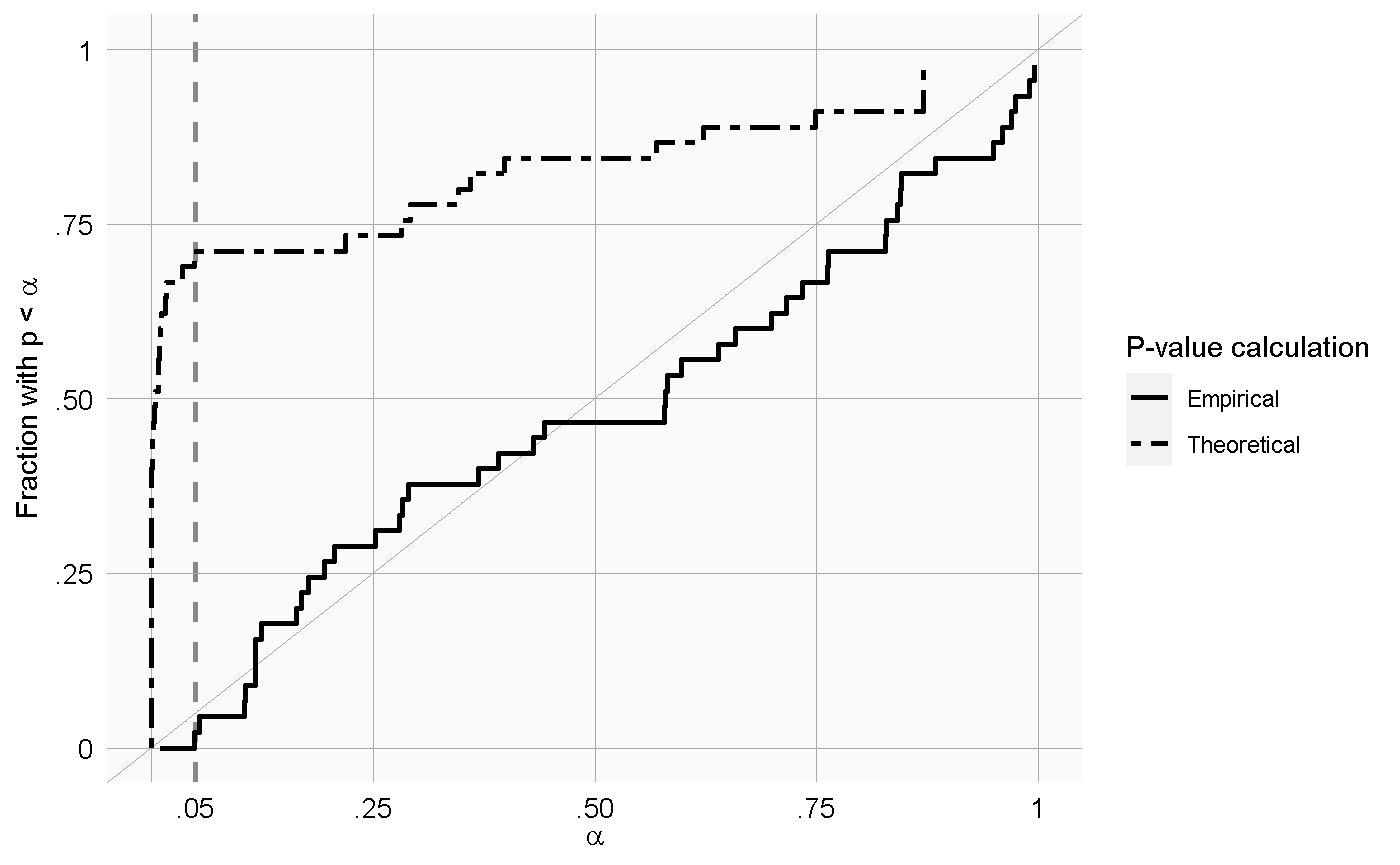
\includegraphics{../inst/doc/EmpiricalCiCalibrationVignette_files/figure-latex/unnamed-chunk-6-1.pdf}

The thick black lines indicate the true effect size, and the blue and
orange dots and lines represent the effect size estimate and 95\%
confidence intervals of the controls. We see that many controls have a
confidence interval that does not include the true effect size (orange
lines), certainly more than the expected 5\%. This indicates the
analysis has systematic error.

\hypertarget{systematic-error-model}{%
\section{Systematic error model}\label{systematic-error-model}}

\hypertarget{fitting-the-empirical-null-and-specifying-an-assumption}{%
\subsection{Fitting the empirical null, and specifying an
assumption}\label{fitting-the-empirical-null-and-specifying-an-assumption}}

If we only have negative controls and no positive controls, we might
still want to calibrate CIs. This requires us to make an assumption how
systematic error changes as a function of the true effect size. The most
obvious (and therefore default) assumption is that the systematic error
does not change as a function of true effect size. We can fit the
empirical null distribution, and convert it to a systematic error model:

\begin{Shaded}
\begin{Highlighting}[]
\NormalTok{null <-}\StringTok{ }\KeywordTok{fitNull}\NormalTok{(negatives}\OperatorTok{$}\NormalTok{logRr, negatives}\OperatorTok{$}\NormalTok{seLogRr)}
\NormalTok{model <-}\StringTok{ }\KeywordTok{convertNullToErrorModel}\NormalTok{(null)}
\end{Highlighting}
\end{Shaded}

See \texttt{?convertNullToErrorModel} for how to use a different
assumption.

\hypertarget{fitting-the-systematic-error-model-using-positive-controls}{%
\subsection{Fitting the systematic error model using positive
controls}\label{fitting-the-systematic-error-model-using-positive-controls}}

If we do have positive controls, like in this example, we do not have to
make an assumption, but instead can estimate the full systematic error
model using the estimates for both negative and positive controls:

\begin{Shaded}
\begin{Highlighting}[]
\NormalTok{model <-}\StringTok{ }\KeywordTok{fitSystematicErrorModel}\NormalTok{(controls}\OperatorTok{$}\NormalTok{logRr, controls}\OperatorTok{$}\NormalTok{seLogRr, controls}\OperatorTok{$}\NormalTok{trueLogRr)}
\NormalTok{model}
\end{Highlighting}
\end{Shaded}

\begin{verbatim}
## meanIntercept     meanSlope   sdIntercept       sdSlope 
##  -0.066550795   0.933292141   0.187468405   0.002979502 
## attr(,"class")
## [1] "systematicErrorModel"
\end{verbatim}

We see that the intercept of the mean (\texttt{meanIntercept}) is
slightly lower than 0, indicating the analysis is negatively biased when
the null is true. Also note that the slope for the mean
(\texttt{meanSlope}) is slightly lower than 1, meaning that the method
appears to be somewhat biased towards the null; the negative bias tends
to become larger as the true effect size increases.

We can also visualize the model:

\begin{Shaded}
\begin{Highlighting}[]
\KeywordTok{plotErrorModel}\NormalTok{(controls}\OperatorTok{$}\NormalTok{logRr, controls}\OperatorTok{$}\NormalTok{seLogRr, controls}\OperatorTok{$}\NormalTok{trueLogRr)}
\end{Highlighting}
\end{Shaded}

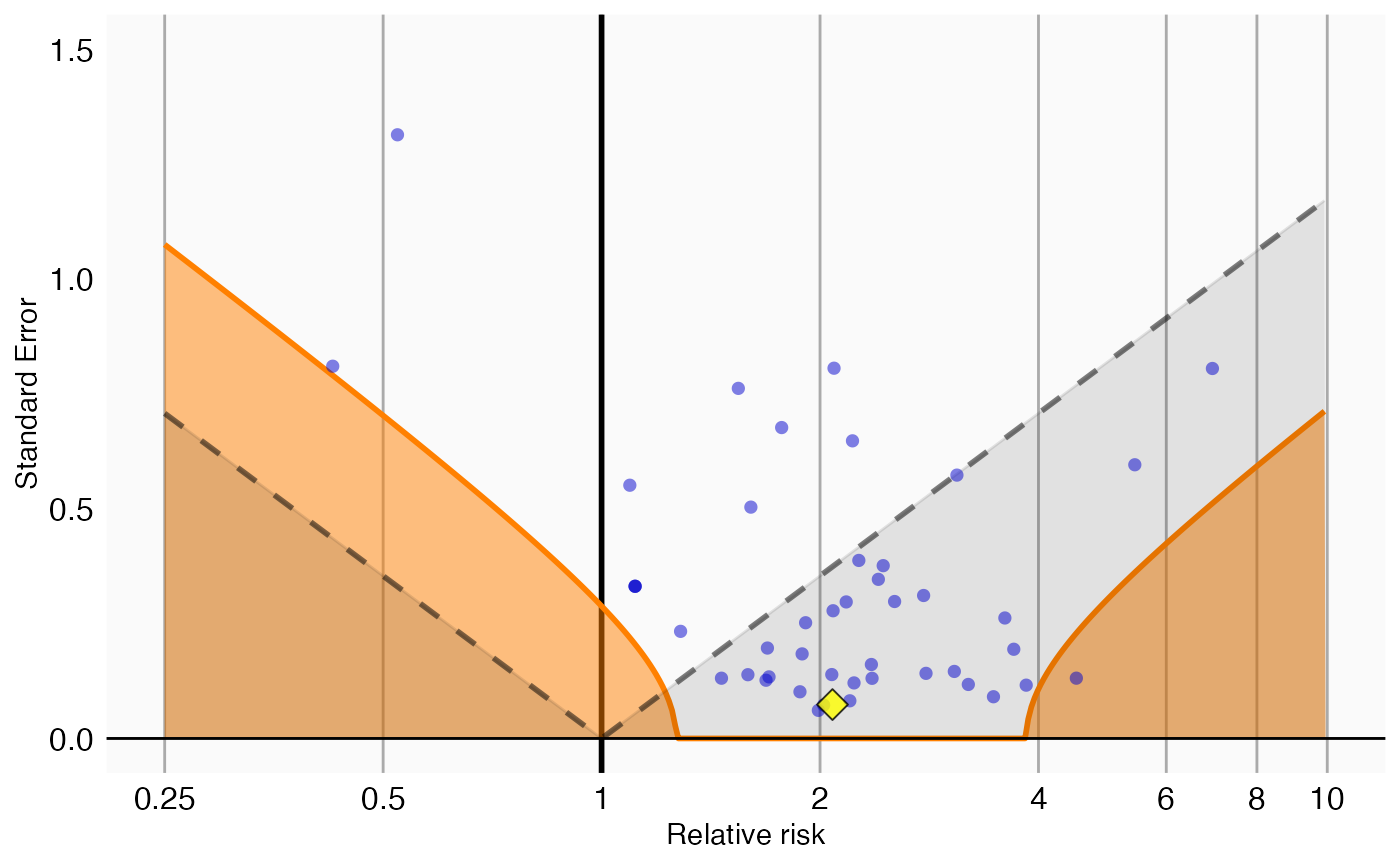
\includegraphics{../inst/doc/EmpiricalCiCalibrationVignette_files/figure-latex/unnamed-chunk-9-1.pdf}

Here we see how systematic error changes as a function of the true
effect size. As visible, the model assumes the mean and standard
deviation (SD) of the error distribution are linearly related to the
true effect size. For this plot, the mean and SD are also estimated at
each true effect size independently, allowing us to evaluate whether the
linearity assumption is far off.

There is also another way to plot the error model, and its subsequent
calibration:

\begin{Shaded}
\begin{Highlighting}[]
\KeywordTok{plotCiCalibrationEffect}\NormalTok{(controls}\OperatorTok{$}\NormalTok{logRr, controls}\OperatorTok{$}\NormalTok{seLogRr, controls}\OperatorTok{$}\NormalTok{trueLogRr)}
\end{Highlighting}
\end{Shaded}

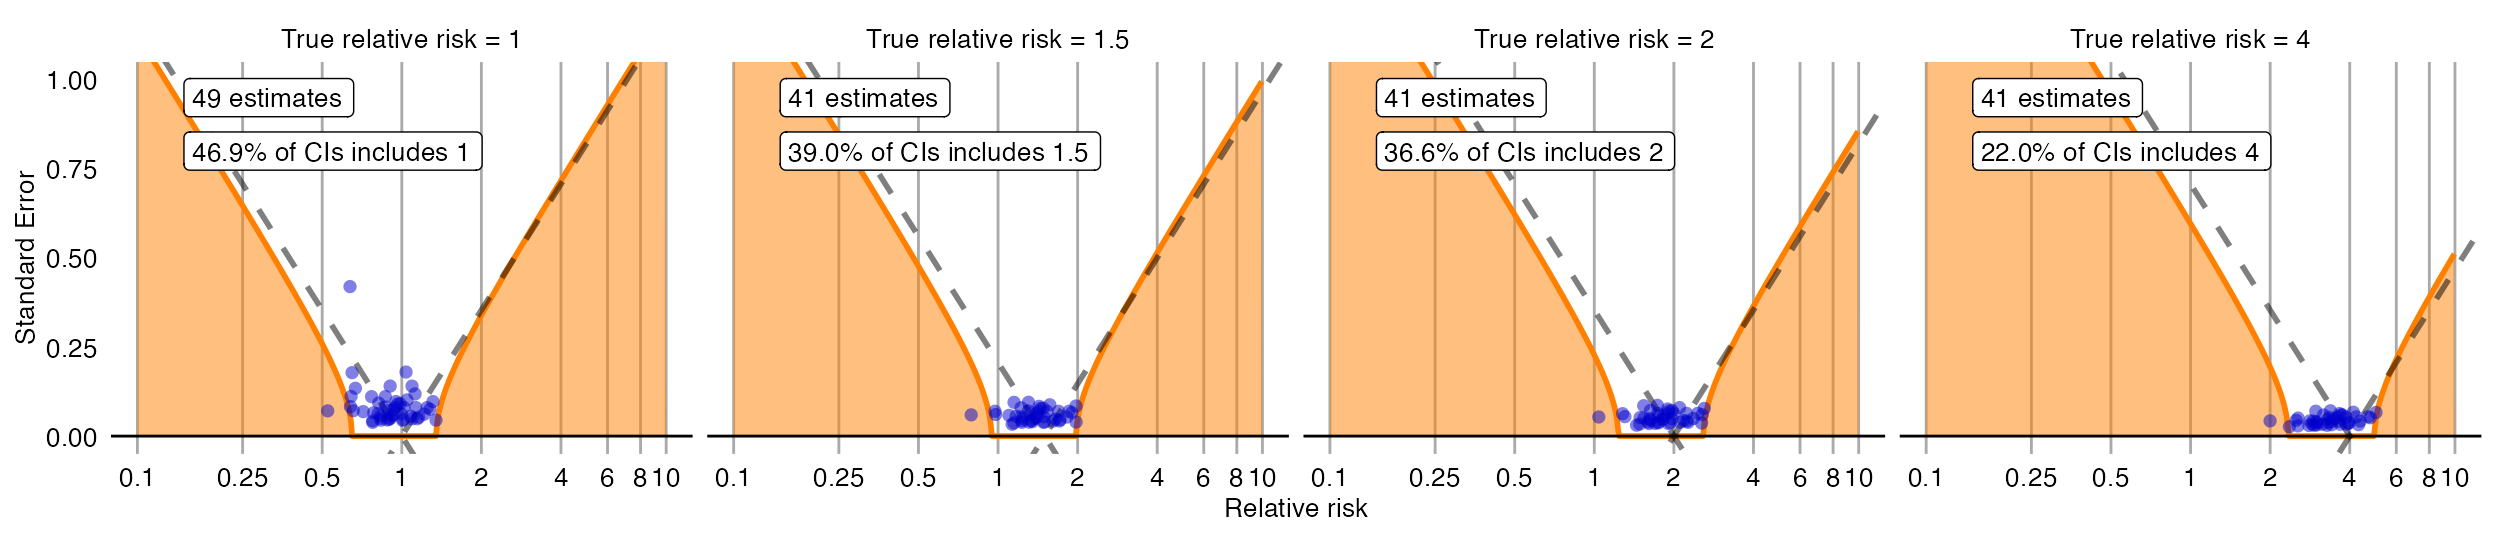
\includegraphics[width=1\linewidth]{../inst/doc/EmpiricalCiCalibrationVignette_files/figure-latex/unnamed-chunk-10-1}

\hypertarget{evaluating-the-calibration}{%
\subsection{Evaluating the
calibration}\label{evaluating-the-calibration}}

To evaluate whether our estimation of the systematic error distribution
is a good one, we can test whether the calibrated CI is truly
calibrated, meaning the fraction of controls where truth is inside the
calibrated CI is approximately the specified width of the CI. We also
evaluate `centeredness', whether truth outside of the CI is equally
distributed above and below the CI:

\begin{Shaded}
\begin{Highlighting}[]
\KeywordTok{plotCiCoverage}\NormalTok{(controls}\OperatorTok{$}\NormalTok{logRr,}
\NormalTok{               controls}\OperatorTok{$}\NormalTok{seLogRr,}
\NormalTok{               controls}\OperatorTok{$}\NormalTok{trueLogRr,}
               \DataTypeTok{crossValidationGroup =}\NormalTok{ controls}\OperatorTok{$}\NormalTok{outcomeName)}
\end{Highlighting}
\end{Shaded}

\begin{verbatim}
## Fitting error models within leave-one-out cross-validation
\end{verbatim}

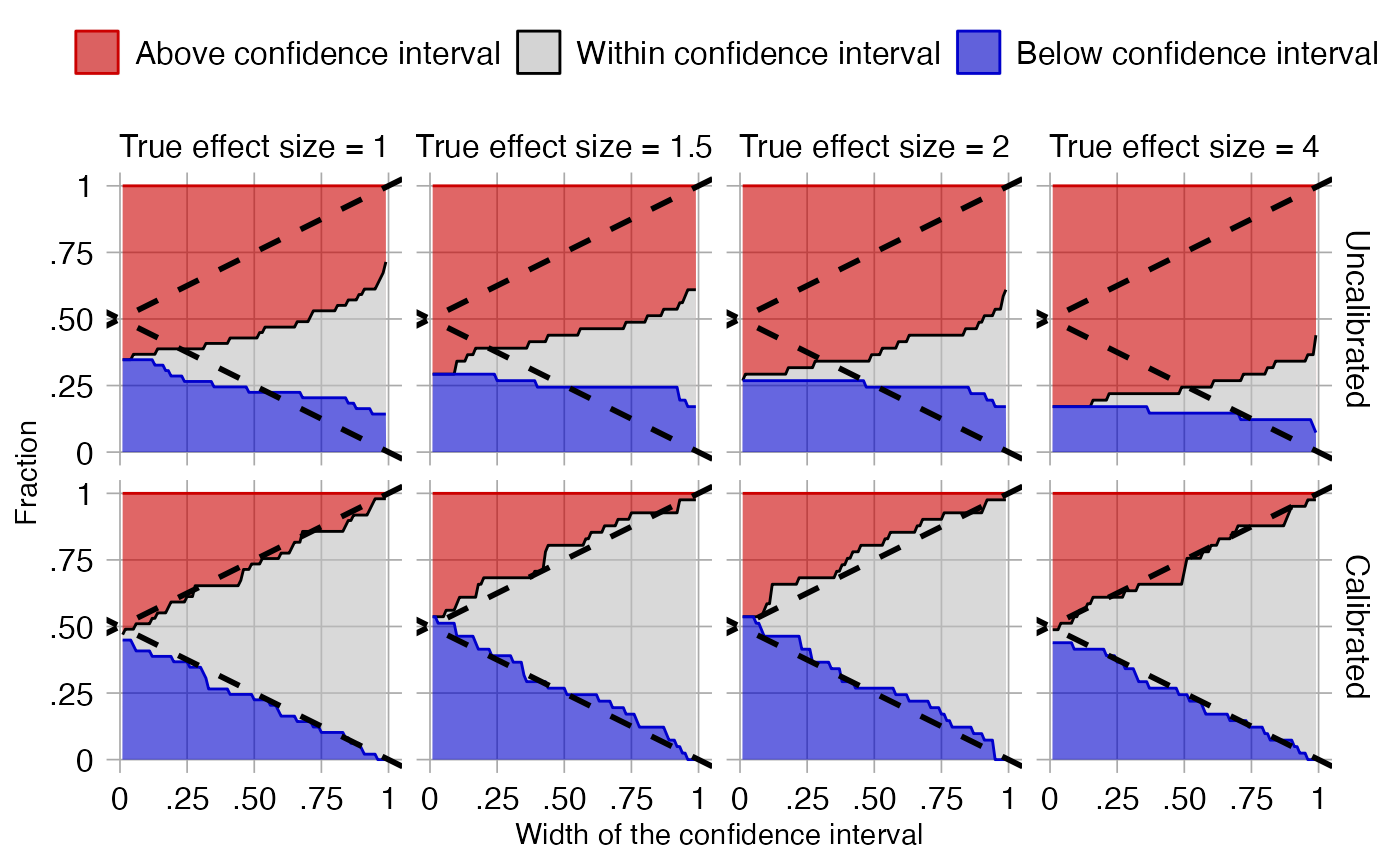
\includegraphics{../inst/doc/EmpiricalCiCalibrationVignette_files/figure-latex/unnamed-chunk-11-1.pdf}

The data shown here is produced using a leave-one-out cross-validation.
It is important to remember that for this dataset positive controls were
generated based on negative controls and will therefore be correlated.
To perform an unbiased evaluation the `one' in the leave-one-out should
therefore be the group of a negative control \emph{and} its derived
positive controls, and this is achieved by specifying the
\texttt{crossValidationGroup} argument. Thus, in this evaluation for
each negative control and the positive controls derived from that
negative control, we fit systematic error models using all other
controls, and compute calibrated CIs for the left-out controls across a
wide range of widths.

In the graph the dashed lines indicate a perfectly calibrated study. We
see that the calibrated CIs are much closer to the ideal than the
uncalibrated CIs.

\hypertarget{confidence-interval-calibration}{%
\section{Confidence interval
calibration}\label{confidence-interval-calibration}}

\hypertarget{calibrating-the-confidence-interval}{%
\subsection{Calibrating the confidence
interval}\label{calibrating-the-confidence-interval}}

We can now use the estimated systematic error model to compute the
calibrated CI for our outcome of interest:

\begin{Shaded}
\begin{Highlighting}[]
\NormalTok{ci <-}\StringTok{ }\KeywordTok{calibrateConfidenceInterval}\NormalTok{(outcomeOfInterest}\OperatorTok{$}\NormalTok{logRr, outcomeOfInterest}\OperatorTok{$}\NormalTok{seLogRr, model)}
\NormalTok{ci}
\end{Highlighting}
\end{Shaded}

\begin{verbatim}
##        logRr logLb95Rr logUb95Rr   seLogRr
## 1 -0.3117702 -0.733957 0.1067054 0.2144587
\end{verbatim}

\begin{Shaded}
\begin{Highlighting}[]
\KeywordTok{exp}\NormalTok{(ci[,}\DecValTok{1}\OperatorTok{:}\DecValTok{3}\NormalTok{])}
\end{Highlighting}
\end{Shaded}

\begin{verbatim}
##       logRr logLb95Rr logUb95Rr
## 1 0.7321498 0.4800058  1.112606
\end{verbatim}

In this case, even though the point estimate has not changed much, the
calibrated CI is much wider than the uncalibrated one to take in to
account the residual error due to lack of any adjustment for
confounding.

\hypertarget{references}{%
\section{References}\label{references}}

\begin{Shaded}
\begin{Highlighting}[]
\KeywordTok{citation}\NormalTok{(}\StringTok{"EmpiricalCalibration"}\NormalTok{)}
\end{Highlighting}
\end{Shaded}

\begin{verbatim}
## 
## To cite EmpiricalCalibration in publications use:
## 
## Schuemie MJ, Ryan PB, DuMouchel W, Suchard MA, Madigan D (2014). "Interpreting observational studies: why
## empirical calibration is needed to correct p-values." _Statistics in Medicine_, *33*(2), 209-218. <URL:
## http://dx.doi.org/10.1002/sim.5925>.
## 
## Schuemie MJ, Hripcsak G, Ryan PB, Madigan D, Suchard MA (2018). "Empirical confidence interval
## calibration for population-level effect estimation studies in observational healthcare data." _Proc.
## Natl. Acad. Sci. U.S.A._, *115*(11), 2571-2577. <URL: https://doi.org/10.1073/pnas.1708282114>.
## 
## To see these entries in BibTeX format, use 'print(<citation>, bibtex=TRUE)', 'toBibtex(.)', or set
## 'options(citation.bibtex.max=999)'.
\end{verbatim}

\end{document}
